\iffalse
\def\mytitle{MATRIX ANALYSIS USING PYTHON}
\def\myauthor{V.GOKULKUMAR}
\def\contact{velicharlagokulkumar@gmail.com}
\def\mymodule{Future Wireless Communication (FWC)}
\documentclass[10pt, a4paper]{article}
\usepackage[a4paper,outer=1.5cm,inner=1.5cm,top=1.75cm,bottom=1.5cm]{geometry}
\twocolumn
\usepackage{graphicx}
\graphicspath{{./images/}}
\usepackage[colorlinks,linkcolor={black},citecolor={blue!80!black},urlcolor={blue!80!black}]{hyperref}
\usepackage[parfill]{parskip}
\usepackage{lmodern}
\usepackage{tikz}
\usepackage{physics}
%\documentclass[tikz, border=2mm]{standalone}
%\usepackage{karnaugh-map}
%\documentclass{article}
\usepackage{tabularx}
%\usepackage{circuitikz}
\usepackage{enumitem}
\usetikzlibrary{calc}
\usepackage{amsmath}
\usepackage{amssymb}
\renewcommand*\familydefault{\sfdefault}
\usepackage{watermark}
\usepackage{lipsum}
\usepackage{xcolor}
\usepackage{listings}
\usepackage{float}
\usepackage{titlesec}
\providecommand{\mtx}[1]{\mathbf{#1}}
\titlespacing{\subsection}{1pt}{\parskip}{3pt}
\titlespacing{\subsubsection}{0pt}{\parskip}{-\parskip}
\titlespacing{\paragraph}{0pt}{\parskip}{\parskip}
\providecommand{\qfunc}[1]{\ensuremath{Q\left(#1\right)}}
\providecommand{\sbrak}[1]{\ensuremath{{}\left[#1\right]}}
\providecommand{\lsbrak}[1]{\ensuremath{{}\left[#1\right.}}
\providecommand{\rsbrak}[1]{\ensuremath{{}\left.#1\right]}}
\providecommand{\brak}[1]{\ensuremath{\left(#1\right)}}
\providecommand{\lbrak}[1]{\ensuremath{\left(#1\right.}}
\providecommand{\rbrak}[1]{\ensuremath{\left.#1\right)}}
\providecommand{\cbrak}[1]{\ensuremath{\left\{#1\right\}}}
\providecommand{\lcbrak}[1]{\ensuremath{\left\{#1\right.}}
\providecommand{\rcbrak}[1]{\ensuremath{\left.#1\right\}}}
\newcommand{\figuremacro}[5]{
    \begin{figure}[H]
        \centering
        \includegraphics[width=0.75\columnwidth]{#2}
        \caption[#3]{\textbf{#3}#4}
        \label{fig:#2}
    \end{figure}
}
\newcommand{\myvec}[1]{\ensuremath{\begin{pmatrix}#1\end{pmatrix}}}
\let\vec\mathbf
\lstset{
frame=single, 
breaklines=true,
columns=fullflexible
}
\thiswatermark{\centering \put(181,-119.0){
\includegraphics[width=0.75\columnwidth]{iith_logo3}} }
\title{\mytitle}
\author{\myauthor\hspace{1em}\\\contact\\FWC22034\hspace{6.5em}IITH\hspace{0.5em}\mymodule\hspace{6em}Assignment}
\begin{document}
	\maketitle
	\tableofcontents
   \section{Problem}
   \fi
   $ABCDE$ is a pentagon. A line through
$\vec{B}$ parallel to $AC$ meets $DC$ produced at $F$. Show
that 
\begin{align}
		\label{eq:9/9/3/11}
	ar (ACB) &= ar (ACF)        
\\
	ar (AEDF) &= ar (ABCDE)
		\label{eq:9/9/3/11/pent}
\end{align}
	\begin{figure}[H]
		\centering
 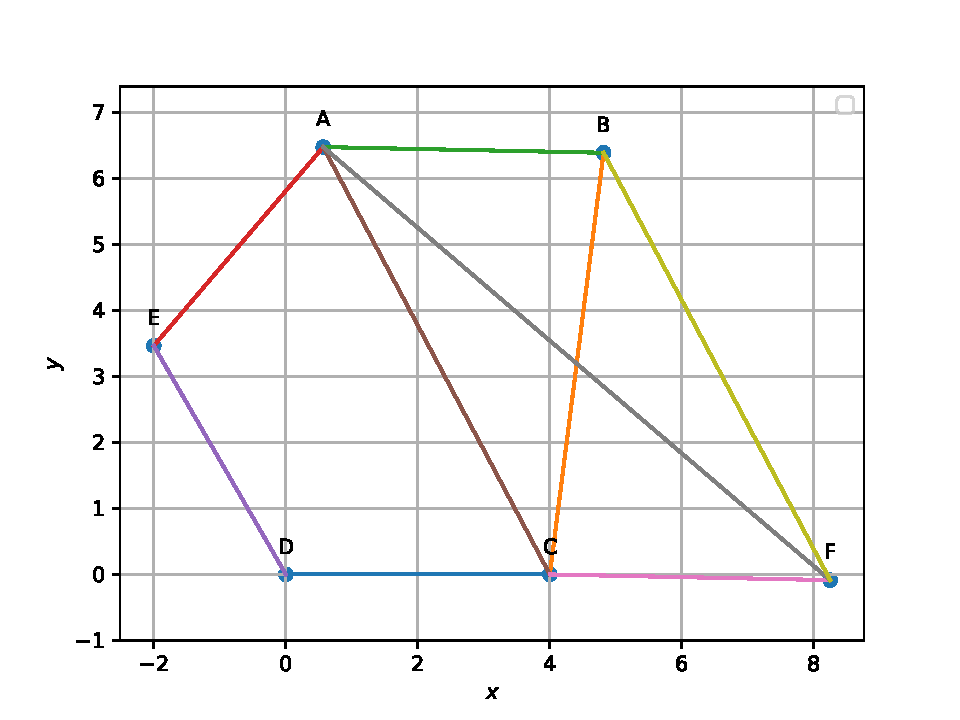
\includegraphics[width=0.75\columnwidth]{chapters/9/9/3/11/figs/matrix.pdf}
		\caption{}
		\label{fig:9/9/3/11}
  	\end{figure}
	\begin{proof}
		Since $BF \parallel AC$,
		\begin{align}
			\vec{F}-\vec{B}&=k\brak{\vec{C}-\vec{A}}
			\\
			\implies \vec{F}&=\vec{B}+k\brak{\vec{C}-\vec{A}}
		\label{eq:9/9/3/11/f}
		\end{align}
		Thus, from  Appendix
  \ref{prop:area2d},
\begin{align}
ar (ACF)
	&= 
 \frac{1}{2}\norm{\vec{F} \times \vec{A}+\vec{A} \times \vec{C}+\vec{C} \times \vec{F}}
%ar (ACB)
% = 
% \frac{1}{2}\norm{\vec{A} \times \vec{B}+\vec{B} \times \vec{C}+\vec{C} \times \vec{A}}
		\label{eq:9/9/3/11/acf}
\end{align}
	Substituting from 
		\eqref{eq:9/9/3/11/f}
		in 
		\eqref{eq:9/9/3/11/acf},
\begin{align}
ar (ACF)
	&= \frac{1}{2}\norm{\cbrak{\vec{B}+k\brak{\vec{C}-\vec{A}}} \times \vec{A}+\vec{A} \times \vec{C}+\vec{C} \times \cbrak{\vec{B}+k\brak{\vec{C}-\vec{A}}}}
	\\
	&= \frac{1}{2}\norm{\vec{B} \times \vec{A}+\vec{A} \times \vec{C}+\vec{C} \times \vec{B}}
	\\
	&= ar\brak{ACB}
\end{align}
upon substituting from		from  Appendix
  \ref{prop:area2d}.
		\eqref{eq:9/9/3/11/pent}
		follows from 
		\eqref{eq:9/9/3/11}.

	\end{proof}

\iffalse

	    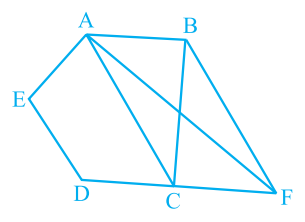
\includegraphics[width=0.75\columnwidth]{diag_1.png}
   \section{Solution}
The input parameters for this construction are 
\begin{center}
\begin{tabular}{|c|c|c|}
	\hline
	\textbf{Symbol}&\textbf{Value}&\textbf{Description}\\
	\hline
	$\vec{D}$ & $\myvec{0\\0}$ & Point D\\
	\hline
	r1&4&DC\\
	\hline
	r2&8&DB\\
	\hline
	r3&6.5&DA\\
	\hline
	r4&4&DE\\
	\hline
	${\theta}_1$& 17$\pi/36$&$ \angle $BDC\\ 
	\hline
	${\theta}_2$& 53$\pi/180$&$ \angle $ADC\\ 
	\hline
	${\theta}_3$& 2$\pi/3$&$ \angle $EDC\\ 
	\hline
\end{tabular}
\end{center}
\begin{center}
Below python code realizes the above construction :
\fbox{\parbox{8.5cm}{\url{https://github.com/velicharlagokulkumar/FWC_module1/blob/main/matrices/lines/codes/matrix.py}}}
\end{center}
\textbf{termux commands :}
\begin{lstlisting}
bash sh.sh.........using shell command
\end{lstlisting}

\textbf{To Prove:} Ar($\vec{A}\vec{C}\vec{B}$)=Ar($\vec{A}\vec{C}\vec{F}$)
\begin{align}
\vec{F}=\vec{C}-\vec{A}+\vec{B}\end{align}
letting
\begin{align}
\vec{v1}=\vec{C}-\vec{A}\\ \vec{v2}=\vec{C}-\vec{F}
\end{align}
Area of the $\Delta \vec{A}\vec{C}\vec{F}$ is given by
\begin{align}
\frac{1}{2} \norm{\vec{v1}\times\vec{v2}}
\end{align}
letting
\begin{align}\vec{v3}=\vec{A}-\vec{C}\\ 
\vec{v4}=\vec{A}-\vec{B}
\end{align}
Area of the $\Delta \vec{A}\vec{C}\vec{B}$ is given by
\begin{align}
\frac{1}{2} \norm{\vec{v3}\times\vec{v4}}
\end{align}
\textbf{To Prove:}  Ar($\vec{A}\vec{E}\vec{D}\vec{F}$)=Ar($\vec{A}\vec{B}\vec{C}\vec{D}\vec{E}$) \\
Area of the $\Delta \vec{A}\vec{E}\vec{D}$ is given by
\begin{align}
\frac{1}{2} \norm{\vec{A}\times\vec{E}}
\end{align}
Area of the $\Delta \vec{A}\vec{D}\vec{C}$ is given by
\begin{align}
\frac{1}{2} \norm{\vec{A}\times\vec{C}}
\end{align}
From (8),(9)
\begin{center}
  Ar($\vec{A}\vec{E}\vec{D}\vec{C}$)=Ar($\Delta$$\vec{A}\vec{E}\vec{D}$)+Ar($\Delta$$\vec{A}\vec{D}\vec{C}$)     \ \ \ \ \ \ \ \ \ \  \ \ \ \ \ \ \ \ \ (10)   
\end{center}
 From (10),(4)
 \begin{center}
$\therefore$ Ar($\vec{A}\vec{E}\vec{D}\vec{F}$)=Ar($\vec{A}\vec{E}\vec{D}\vec{C}$)+Ar($\Delta$$\vec{A}\vec{C}\vec{F}$)
\end{center}
 From (10),(7)
 \begin{center}
$\therefore$ Ar($\vec{A}\vec{B}\vec{C}\vec{D}\vec{E}$)=Ar($\vec{A}\vec{E}\vec{D}\vec{C}$)+Ar($\Delta$$\vec{A}\vec{C}\vec{B}$)
\end{center}
 \section{Construction}
 	\begin{center}
  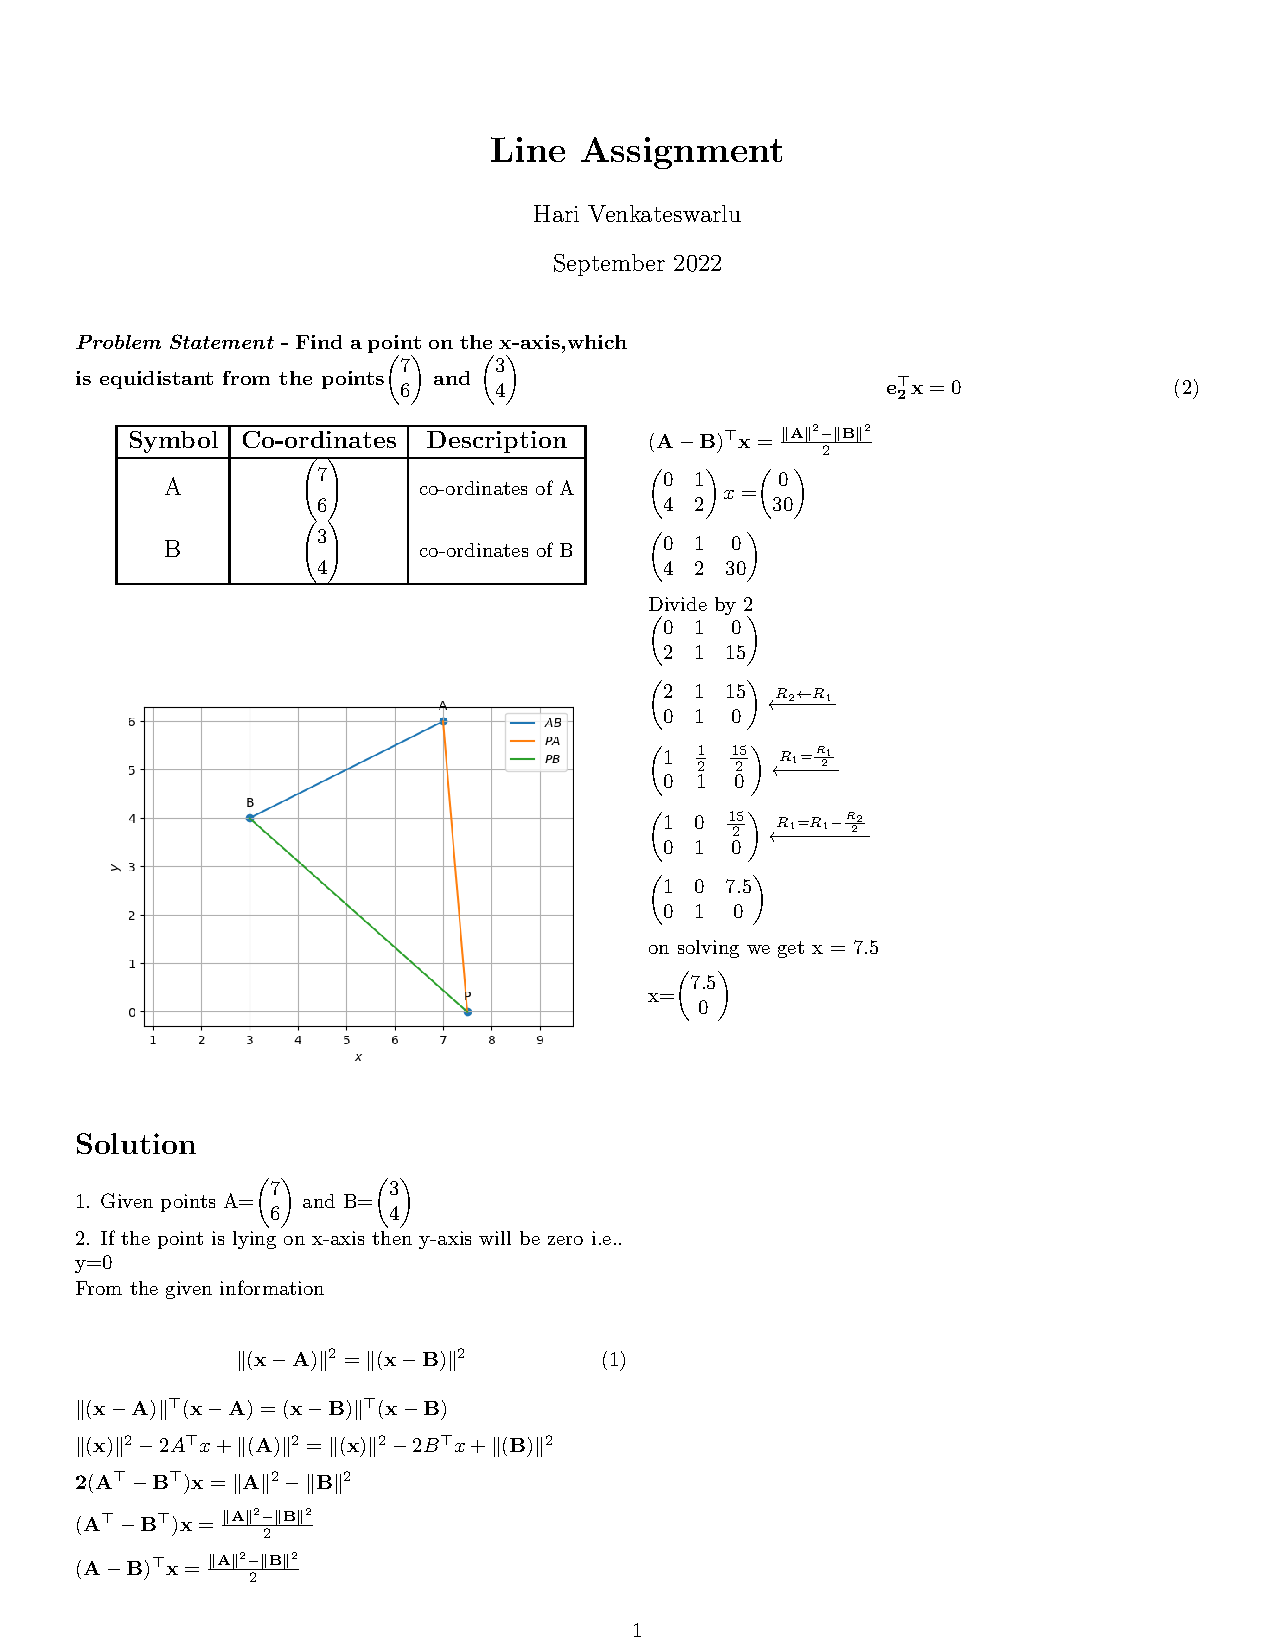
\includegraphics[width=0.75\columnwidth]{matrix.pdf}\\
       Figure of construction 
  	\end{center}
\end{document}
\fi
